% ---------------------------------------------------------------------------
% dendritic_credit_workshop_core.tex — core slides (35 frames).
% Technical workshop deck, revised to the one-deck brief: one idea and one
% visual anchor per slide, hero equations (\heroeq + \term anatomy), one
% large semantic headline number, schematics first, act dividers as
% questions. Every equation is copied verbatim (up to display arrangement)
% from journal main.tex; numbers come from journal main.tex or
% dendritic_credit_expanded_core.tex. Secondary statistics removed from the
% slides live in speaker_notes_workshop.md.
% Keep \CoreSlides in dendritic_credit_workshop.tex in sync with the count.
% ---------------------------------------------------------------------------

% ===========================================================================
% ACT I — Learning as a credit-assignment problem
% ===========================================================================

% 1 — title slide
\begin{frame}
  \begin{columns}[c,onlytextwidth]
    \begin{column}{0.66\textwidth}
      {\color{Shunt}\rule{1.15cm}{1.6pt}}\par
      \vspace{0.34cm}
      {\fontsize{26}{31}\selectfont\bfseries What dendritic structure\\[0.06cm]adds to learning\par}
      \vspace{0.34cm}
      {\normalsize\color{Mute}Credit assignment from neurons to branches: coordinates, subtree addresses and route gain\par}
      \vspace{0.60cm}
      {\small Houman Safaai\enspace\textperiodcentered\enspace Maceo Richards\enspace\textperiodcentered\enspace Bernardo L. Sabatini\par}
      \vspace{0.10cm}
      {\footnotesize\color{Mute}Kempner Institute, Harvard University\enspace\textperiodcentered\enspace Harvard Medical School\par}
      \vspace{0.30cm}
      {\footnotesize\color{Mute}Kempner Learning Dynamics Workshop\enspace\textperiodcentered\enspace 2026\par}
    \end{column}
    \begin{column}{0.30\textwidth}
      \centering
      \dendtree[1.62]
    \end{column}
  \end{columns}
\end{frame}

% 2 — the hook: one error, ten thousand synapses
\begin{frame}{One error arrives. Ten thousand synapses must decide.}
  \begin{columns}[c,onlytextwidth]
    \begin{column}{0.44\textwidth}
      \headline[Shunt]{$\sim\!10^{4}$}{synapses arrayed on one branching
        arbor}
      \vspace{0.34cm}
      {\small Which of them should change, in which direction, by how
       much?\par}
      \vspace{0.22cm}
      {\footnotesize\color{Mute}The task delivers one output error --- at the
       soma.\par}
    \end{column}
    \begin{column}{0.52\textwidth}
      \centering
      \CreditTree[mode=plain,scale=1.18,stagelabel={one output error arrives at the soma}]
    \end{column}
  \end{columns}
  \vfill
  \takeaway{The tree between soma and synapse is either in the way --- or part of the answer.}
  \vspace{0.04cm}
\end{frame}

% 3 — learning dynamics reduce to credit
\begin{frame}{Learning dynamics reduce to who gets credit}
  \begin{columns}[T,onlytextwidth]
    \begin{column}{0.36\textwidth}
      \centering
      \vspace{0.30cm}
      \begin{tikzpicture}[line cap=round]
        % three layers of three units
        \foreach \x/\n in {0/a,1.45/b,2.90/c}{
          \foreach \y/\k in {0/1,0.75/2,1.50/3}{
            \node[circle,draw=Mute,fill=Paper,line width=0.6pt,inner sep=0pt,
                  minimum size=8.5pt] (\n\k) at (\x,\y) {};
          }}
        \foreach \i in {1,2,3}\foreach \j in {1,2,3}{
          \draw[Grid,line width=0.55pt] (a\i) -- (b\j);
          \draw[Grid,line width=0.55pt] (b\i) -- (c\j);}
        \node[rounded corners=2pt,draw=Ink!40,fill=Paper,inner sep=2.6pt,
              font=\scriptsize] (loss) at (4.05,0.75) {$\mathcal L$};
        \draw[Mute,line width=0.7pt] (c2) -- (loss);
        % backward error flow
        \draw[BP,-{Stealth[length=4pt]},line width=0.9pt]
          (3.90,0.42) to[bend left=22] (3.05,0.14);
        \draw[BP,-{Stealth[length=4pt]},line width=0.9pt]
          (2.70,-0.28) to[bend left=14] (1.62,-0.28);
        \draw[BP,-{Stealth[length=4pt]},line width=0.9pt]
          (1.25,-0.28) to[bend left=14] (0.17,-0.28);
        \node[font=\tiny,text=BP,anchor=south] at (1.68,1.86) {$\bm\delta^{\ell}$};
        \draw[BP,-{Stealth[length=3.5pt]},line width=0.7pt]
          (1.66,1.84) -- (1.52,1.62);
        \node[font=\tiny,text=Mute,anchor=north] at (1.45,-0.66)
          {error flows backward, layer by layer};
      \end{tikzpicture}
    \end{column}
    \begin{column}{0.60\textwidth}
      \heroeq[gradient flow]{%
        \begin{gathered}
          \frac{\dd\bm\theta}{\dd t}=-\eta\,\nabla_{\bm\theta}\mathcal L
          \\[0.42cm]
          \frac{\partial\mathcal L}{\partial W^{\ell}_{ji}}
          =\term[Shunt]{h^{\ell-1}_i\vphantom{\delta^{\ell}_j}}{presynaptic input}\,
           \term[Add]{\delta^{\ell}_j\vphantom{h^{\ell-1}_i}}{destination error}
        \end{gathered}}
      \vspace{0.06cm}
      \deftag{sign}\enspace{\footnotesize potentiate or depress}\par
      \vspace{0.10cm}
      \deftag{magnitude}\enspace{\footnotesize how strongly this parameter moves the loss}\par
      \vspace{0.10cm}
      \deftag{destination}\enspace{\footnotesize every parameter indexed exactly}\par
    \end{column}
  \end{columns}
  \vfill
  \takeaway{A theory of biological learning must say what stands in for $\bm\delta$ at each synapse.}
  \vspace{0.04cm}
\end{frame}

% 4 — BP as reference, and the local template
\begin{frame}{Backprop is the reference, not the mechanism}
  \heroeq[backprop update]{%
    \Delta W^{\ell}_{ji}=-\eta\,h^{\ell-1}_i\delta^{\ell}_j,
    \qquad
    \bm\delta^{\ell}
    =\term[BP]{(W^{\ell+1})^{\mathsf T}\bm\delta^{\ell+1}}{weight transport}
     \odot f'(\bm a^{\ell})}
  \vspace{0.16cm}
  \begin{columns}[c,onlytextwidth]
    \begin{column}{0.30\textwidth}
      {\scriptsize\color{Mute}what backprop demands\par}
      \vspace{0.12cm}
      \deftag{transport}\par
      \vspace{0.14cm}
      \deftag{coordination}\par
      \vspace{0.14cm}
      \deftag{nonlocal state}\par
    \end{column}
    \begin{column}{0.40\textwidth}
      {\footnotesize\good{a synapse sees:} input, compartment state, one
       teaching signal.\par}
    \end{column}
    \begin{column}{0.24\textwidth}
      \centering
      \CreditTree[mode=plain,scale=0.62]
    \end{column}
  \end{columns}
  \vfill
  \takeaway{Judge every biological rule by the information it puts in place of $\bm\delta$.}
  \vspace{0.04cm}
\end{frame}

% 5 — ACT II divider
\begin{frame}[t]
  \vspace{1.55cm}
  {\color{Shunt}\bfseries\scriptsize ACT II\par}
  \vspace{0.30cm}
  {\fontsize{20}{25}\selectfont\bfseries\color{Ink}Which neuron should change?\par}
  \vspace{0.28cm}
  {\small\color{Mute}The state of the art, read analytically\par}
  \vfill
  \hfill\stackmotif{1}\par
  \vspace{0.12cm}
\end{frame}

% ===========================================================================
% ACT II — State of the art, analytically
% ===========================================================================

% 6 — taxonomy
\begin{frame}{Four families of answers}
  \begin{columns}[T,onlytextwidth]
    \begin{column}{0.485\textwidth}
      \claimbox{%
        \deftag{scalar modulator}\par
        \vspace{-0.08cm}
        {\small\[\Delta w_i\propto e_i\,m_u\]\par}
        \vspace{-0.18cm}
        {\scriptsize\color{Mute}Fr\'emaux \& Gerstner 2016\par}}
      \vspace{0.16cm}
      \claimbox{%
        \deftag{state inference}\par
        \vspace{0.05cm}
        {\footnotesize teaching signal $=$ nudged-state difference\par}
        \vspace{0.05cm}
        {\scriptsize\color{Mute}Scellier \& Bengio 2017; Whittington \&
         Bogacz 2017\par}}
    \end{column}
    \begin{column}{0.485\textwidth}
      \claimbox{%
        \deftag{random feedback coordinate}\par
        \vspace{-0.08cm}
        {\small\[\widehat{\bm\delta}^{\ell}=B^{\ell}\bm\delta^{\mathrm{out}}\]\par}
        \vspace{-0.18cm}
        {\scriptsize\color{Mute}Lillicrap et al.\ 2016; N\o kland 2016\par}}
      \vspace{0.16cm}
      \claimbox{%
        \deftag{dendritic error compartments}\par
        \vspace{0.05cm}
        {\footnotesize one error per neuron, held beside its activity\par}
        \vspace{0.05cm}
        {\scriptsize\color{Mute}Guerguiev et al.\ 2017; Sacramento et al.\
         2018; Payeur et al.\ 2021; Song et al.\ 2024\par}}
    \end{column}
  \end{columns}
  \vfill
  \takeaway{Each family delivers a different error to the neuron; none indexes a branch.}
  \vspace{0.04cm}
\end{frame}

% 7 — convergence on a per-neuron coordinate
\begin{frame}{They converge on one per-neuron coordinate $\delta_u$}
  \begin{columns}[T,onlytextwidth]
    \begin{column}{0.60\textwidth}
      {\scriptsize\color{Mute}point neuron:
       $s_u=\sum_i w_ix_i$, \ $V_u=f(s_u)$\par}
      \heroeq[point neuron]{%
        \frac{\partial\mathcal L}{\partial w_i}
        =\term[Shunt]{x_if'(s_u)}{synapse-local eligibility}\;
         \term[Add]{\delta_u\vphantom{x_if'(s_u)}}{one shared coordinate}}
      \vspace{0.10cm}
      {\footnotesize No variable in this equation can address one subtree
       differently from another.\par}
    \end{column}
    \begin{column}{0.36\textwidth}
      \centering
      \CreditTree[mode=coordinate,scale=1.02,stagelabel={credit stops at the soma}]
    \end{column}
  \end{columns}
  \vfill
  \takeaway{Point-based theories have no addressable variable inside the arbor.}
  \vspace{0.04cm}
\end{frame}

% 8 — this talk
\begin{frame}{This talk: what does the tree add after $\delta_{0,u}$ arrives?}
  \heroeq*[preview]{%
    \frac{\partial\mathcal L}{\partial g_i}
    =\term[Shunt]{e_i\vphantom{\widetilde\alpha_{n(i)}}}{local state}\;
     \term[Add]{\delta_{0,u}\vphantom{\widetilde\alpha_{n(i)}}}{neuron
       coordinate}\;
     \term[Dend]{\widetilde\alpha_{n(i)}}{address and route gain}}
  \vspace{0.08cm}
  \centering
  \TreeStrip{\CreditTree[mode=coordinate,scale=0.58,stagelabel={coordinate}]}%
            {\CreditTree[mode=address,K=4,scale=0.58,stagelabel={address}]}%
            {\CreditTree[mode=gain,scale=0.58,stagelabel={gain}]}\par
  \vfill
  \raggedright
  \takeaway{Three candidate roles for the tree: local state, subtree addresses, route gains.}
  \vspace{0.04cm}
\end{frame}

% 9 — ACT III divider
\begin{frame}[t]
  \vspace{1.55cm}
  {\color{Shunt}\bfseries\scriptsize ACT III\par}
  \vspace{0.30cm}
  {\fontsize{20}{25}\selectfont\bfseries\color{Ink}What exactly does a tree add\\[0.04cm]to a teaching signal?\par}
  \vspace{0.28cm}
  {\small\color{Mute}Theory: eligibility, transport, capture, bandwidth and gain\par}
  \vfill
  \hfill\stackmotif{2}\par
  \vspace{0.12cm}
\end{frame}

% ===========================================================================
% ACT III — Theory of dendritic credit
% ===========================================================================

% 10 — forward model
\begin{frame}{The forward model is a conductance quotient}
  \heroeq[model]{%
    V_n=\term[Shunt]{R_n^{\mathrm{tot}}}{conductance quotient}
      \Bigl(\sum_{i\in\mathcal S_n}g_ix_iE_i
        +\sum_{c\in\mathcal C_n}g^{\mathrm{den}}_{c\to n}a_c
        +g_n^LE_L\Bigr)}
  \begin{columns}[T,onlytextwidth]
    \begin{column}{0.58\textwidth}
      {\scriptsize\color{Mute}
       $R_n^{\mathrm{tot}}=(g_n^{\mathrm{tot}})^{-1},\quad
        g_n^{\mathrm{tot}}=g_n^L+\sum_{i\in\mathcal S_n}g_ix_i
          +\sum_{c\in\mathcal C_n}g^{\mathrm{den}}_{c\to n}$\par}
      \vspace{0.18cm}
      {\footnotesize Every input raises both the weighted drive and the total
       conductance.\par}
      \srcnote{Journal Eq.~5 (steady-state compartment equation);
        $a_c=f_c(V_c)$ propagates rootward.}
    \end{column}
    \begin{column}{0.38\textwidth}
      \centering
      \CreditTree[mode=forward,scale=0.78,stagelabel={state carried at every compartment}]
    \end{column}
  \end{columns}
  \vfill
  \takeaway{The quotient is the mechanism: normalization lives in the denominator.}
  \vspace{0.04cm}
\end{frame}

% 11 — eligibility
\begin{frame}{The quotient rule yields an exact local eligibility}
  \begin{columns}[T,onlytextwidth]
    \begin{column}{0.62\textwidth}
      \heroeq[exact local eligibility]{%
        \frac{\partial V_n}{\partial g_i}
        =\term[Shunt]{x_i\vphantom{(E_i-V_n)}}{presynaptic activity}\,
         \term[Shunt]{R_n^{\mathrm{tot}}\vphantom{(E_i-V_n)}}{input
           resistance}\,
         \term[Shunt]{(E_i-V_n)}{driving force}
        \;\equiv\;e_i}
      \vspace{0.10cm}
      {\footnotesize The quotient rule creates the driving-force factor;
       additive-current models lose it.\par}
      \srcnote{Journal Eq.~6; full quotient-rule steps in backup.}
    \end{column}
    \begin{column}{0.34\textwidth}
      \centering
      \CreditTree[mode=eligibility,scale=0.80,stagelabel={the three local factors of $e_i$}]
    \end{column}
  \end{columns}
  \vfill
  \takeaway{Conductance normalization does not destroy locality; it creates the exact factor $E_i-V_n$.}
  \vspace{0.04cm}
\end{frame}

% 12 — factorization + transport
\begin{frame}{Every exact gradient factors: eligibility $\times$ transported error}
  \begin{columns}[T,onlytextwidth]
    \begin{column}{0.62\textwidth}
      \heroeq[theorem]{%
        \begin{gathered}
          \frac{\partial\mathcal L}{\partial g_i}
          =\term[Shunt]{e_i\vphantom{\delta_n}}{local eligibility}\,
           \term[Add]{\delta_n\vphantom{e_i}}{transported error},
          \quad
          \delta_n=\delta_{0,u}\,\widetilde\alpha_n
          \\[0.58cm]
          \widetilde\alpha_n
          =\prod_{(i\to k)\in\operatorname{path}(n\to0)}
            f_i'(V_i)\,R_k^{\mathrm{tot}}\,g^{\mathrm{den}}_{i\to k}
        \end{gathered}}
      \srcnote{Journal Eqs.~2--4 and 6--7; exact reconstruction matched
        autodiff on every diagnostic run.}
    \end{column}
    \begin{column}{0.34\textwidth}
      \centering
      \CreditTree[mode=transport,scale=0.94,stagelabel={one route from soma to every site}]
    \end{column}
  \end{columns}
  \vfill
  \takeaway{Every biological proposal is an explicit approximation to the transported factor $\delta_n$.}
  \vspace{0.04cm}
\end{frame}

% 13 — the four-level hierarchy (map slide)
\begin{frame}{Dendritic credit is a four-level hierarchy of error fields}
  \centering
  \vspace{0.14cm}
  % rank labels ride inside each stagelabel (\shortstack), so every label is
  % optically centered under its own tree's soma.
  \TreeStrip{\CreditTree[mode=scalar,scale=0.58,stagelabel={\shortstack{global
              scalar\\[1.5pt]{\color{Amber}\bfseries rank-0 broadcast}}}]}%
            {\CreditTree[mode=coordinate,scale=0.58,stagelabel={\shortstack{neuron
              coordinate\\[1.5pt]{\color{Add}\bfseries rank-1 per neuron}}}]}%
            {\CreditTree[mode=address,K=4,scale=0.58,stagelabel={\shortstack{subtree
              address\\[1.5pt]{\color{Dend}\bfseries rank-$K$ nested routes}}}]}%
            {\CreditTree[mode=gain,scale=0.58,stagelabel={\shortstack{route
              gain\\[1.5pt]{\color{Shunt}\bfseries reliability-weighted}}}]}\par
  \vfill
  \raggedright
  \takeaway{This ladder is the map of the talk: each experiment tests one rung against the next.}
  \vspace{0.04cm}
\end{frame}

% 14 — stochastic credit operator
\begin{frame}{A stochastic credit operator predicts when routes help}
  {\scriptsize\color{Mute}update
   $\bm w^{+}=\bm w-\eta M\widehat{\bm g}$, teaching field
   $\widehat{\bm g}=\bm g+\bm\xi$, noise covariance $\Sigma$\par}
  \heroeq[descent bound and phase utility]{%
    \begin{gathered}
      \E\,\mathcal L(\bm w^{+})\leq\mathcal L(\bm w)
        -\eta\,\term[Shunt]{\bm g^{\mathsf T}M\bm g}{retained signal}
        +\frac{L\eta^{2}}{2}\Bigl(
          \term[Amber]{\lVert M\bm g\rVert_2^{2}}{curvature bias}
          +\term[BP]{\tr(M\Sigma M^{\mathsf T})}{admitted noise}\Bigr)
      \\[0.66cm]
      U(M)=\frac{[\bm g^{\mathsf T}M\bm g]^{2}}
        {2L\bigl\{\lVert M\bm g\rVert_2^{2}
          +\tr(M\Sigma M^{\mathsf T})\bigr\}},
      \qquad \bm g^{\mathsf T}M\bm g>0
    \end{gathered}}
  \vspace{0.04cm}
  {\footnotesize Positivity is the feedback-alignment condition; the bound is
   exact for the matched quadratic.\ {\color{Mute}Journal Eqs.~8--9.}\par}
  \vfill
  \takeaway{A restricted route helps exactly when retained signal beats bias plus admitted noise.}
  \vspace{0.04cm}
\end{frame}

% 15 — capture and tree spectrum
\begin{frame}{Capture and the tree spectrum pick the best dictionary}
  \begin{columns}[T,onlytextwidth]
    \begin{column}{0.55\textwidth}
      \heroeq[capture]{%
        \term[Dend]{\mathcal C_K(\bm g;\Phi,W)
          =\frac{\lVert\overline P_{\Phi}\overline{\bm g}\rVert_2^{2}}
                {\lVert\overline{\bm g}\rVert_2^{2}}}{task-gradient energy
            inside the anatomical span}}
      {\scriptsize\color{Mute}spectral form:
       $\mathcal C_K(\overline C_g)
        =\tr(\overline P_{\Phi}\overline C_g)/\tr(\overline C_g)$;
       ancestry spans the $K$ coarsest tree-Haar modes\par}
      \headline[Shunt]{$+0.55$}{more captured task energy than a random
        rank-matched route --- ancestry at $K{=}4$ under full task--tree
        alignment, 50/50 seeds}
    \end{column}
    \begin{column}{0.41\textwidth}
      \centering
      \begin{tikzpicture}[line cap=round]
        \draw[Mute,line width=0.6pt] (-0.15,0) -- (4.35,0);
        \foreach \i/\h/\c in {1/2.00/Shunt,2/1.44/Shunt,3/1.10/Shunt,4/0.84/Shunt,
                              5/0.36/Grid,6/0.26/Grid,7/0.20/Grid,8/0.16/Grid}{
          \pgfmathsetmacro{\x}{0.52*(\i-1)+0.10}
          \fill[\c] (\x,0) rectangle ({\x+0.34},\h);}
        \draw[decorate,decoration={brace,amplitude=3.5pt},Ink,line width=0.6pt]
          (0.06,2.14) -- (2.10,2.14);
        \node[font=\tiny,text=Ink,anchor=south] at (1.08,2.30)
          {ancestry span, $K=4$};
        \node[font=\tiny,text=Mute,anchor=north] at (2.10,-0.10)
          {tree-Haar modes, coarse $\to$ fine};
        \node[font=\tiny,text=Mute,anchor=east,rotate=90] at (-0.24,2.05)
          {task-credit spectrum};
      \end{tikzpicture}\par
      \vspace{0.12cm}
      {\scriptsize\color{Mute}coarse-dominant spectrum $\Rightarrow$ the
       anatomical span is Ky--Fan optimal\par}
    \end{column}
  \end{columns}
  \vfill
  \takeaway{Anatomy is optimal when task covariance is coarse-dominant in the tree's own basis.}
  \vspace{0.04cm}
\end{frame}

% 16 — interior optimum
\begin{frame}{Bandwidth has an interior optimum}
  \begin{columns}[T,onlytextwidth]
    \begin{column}{0.50\textwidth}
      \heroeq[projection beats full bandwidth iff]{%
        \term[BP]{\tr[(I-P)\Sigma]\vphantom{\lVert(I-P)\bm
          g\rVert_2^{2}}}{rejected noise}
        \;>\;
        \term[Add]{\lVert(I-P)\bm g\rVert_2^{2}}{discarded signal}}
      {\scriptsize\color{Mute}identity-curvature quadratic at
       $\eta=1/L$\par}
      \vspace{0.14cm}
      {\footnotesize Bandwidth pays only while each added route scale brings
       more signal than admitted noise.\par}
    \end{column}
    \begin{column}{0.46\textwidth}
      \centering
      % conceptual regime plane, drawn native at slide font sizes; the
      % measured phase plane closes the talk in Act V
      \begin{tikzpicture}[line cap=round]
        \fill[Paper]    (0,0)    rectangle (5.70,3.70);
        \fill[BP!7]     (0,2.85) rectangle (5.70,3.70);
        \fill[Amber!16] (0,0)    rectangle (5.70,0.55);
        \begin{scope}
          \clip (0,0.55) rectangle (5.70,2.85);
          \fill[ShuntPale] (2.75,0.55) .. controls (2.35,1.70) .. (2.05,2.85)
            -- (5.70,2.85) -- (5.70,0.55) -- cycle;
        \end{scope}
        \draw[Mute,line width=0.5pt,dash pattern=on 1.6pt off 1.4pt]
          (2.75,0.55) .. controls (2.35,1.70) .. (2.05,2.85);
        \draw[Mute,line width=0.5pt,dash pattern=on 1.6pt off 1.4pt]
          (0,2.85) -- (5.70,2.85);
        \node[font=\tiny,text=Mute,anchor=west] at (3.95,3.00)
          {$K=r_{\mathrm{eff}}$};
        \node[font=\scriptsize,text=Mute] at (3.10,3.48)
          {spans coincide: routing ties exact};
        \node[font=\scriptsize,text=Mute,align=center] at (1.10,2.05)
          {low-rank random\\routes win};
        \node[font=\scriptsize,text=Shunt!55!Ink,align=center] at (4.30,1.30)
          {anatomical\\routes win};
        \node[font=\tiny,text=Amber!50!Ink] at (2.85,0.28)
          {too few channels: identity binds};
        \draw[Mute,line width=0.6pt] (0,0) -- (5.70,0);
        \draw[Mute,line width=0.6pt] (0,0) -- (0,3.70);
        \node[font=\scriptsize,text=Ink,anchor=north] at (2.85,-0.08)
          {task--anatomy alignment $0\to1$};
        \node[font=\scriptsize,text=Ink,anchor=south,rotate=90]
          at (-0.14,1.85) {bandwidth $K/r_{\mathrm{eff}}$};
      \end{tikzpicture}\par
      \vspace{0.08cm}
      {\scriptsize\color{Mute}conceptual regime bands, not fitted --- the
       measured plane closes the talk\par}
    \end{column}
  \end{columns}
  \vfill
  \takeaway{This phase plane sets up every experiment in the next act.}
  \vspace{0.04cm}
\end{frame}

% 17 — reliability-weighted route gain
\begin{frame}{Conductance implements reliability-weighted route gain}
  \begin{columns}[T,onlytextwidth]
    \begin{column}{0.34\textwidth}
      \centering
      \CreditTree[mode=gain,scale=0.95,stagelabel={stroke width $=$ route gain}]
    \end{column}
    \begin{column}{0.62\textwidth}
      \heroeq[optimal branch attenuation]{%
        a_b^{*}=\min\Bigl\{1,\;
          \term[Shunt]{S_b\vphantom{c\,(S_b+N_b)}}{branch signal}
          \bigm/
          \term[BP]{c\,(S_b+N_b)}{dose $\times$ (signal $+$ noise)}
        \Bigr\}}
      \vspace{0.10cm}
      {\footnotesize A shunt is a rank-one conductance edit of the adjoint
       (Sherman--Morrison); dose raises its amplitude monotonically, then
       saturates.\par}
      \srcnote{Journal, credit-operator section; rank-one identity and
        selectivity criterion in backup.}
    \end{column}
  \end{columns}
  \vfill
  \takeaway{Branch-local conductance can realize the optimal attenuation $a_b^{*}$ --- physically and locally.}
  \vspace{0.04cm}
\end{frame}

% 18 — ACT IV divider
\begin{frame}[t]
  \vspace{1.55cm}
  {\color{Shunt}\bfseries\scriptsize ACT IV\par}
  \vspace{0.30cm}
  {\fontsize{20}{25}\selectfont\bfseries\color{Ink}Do subtree addresses and route gains\\[0.04cm]actually pay?\par}
  \vspace{0.28cm}
  {\small\color{Mute}A battery of matched experiments, one rung at a time\par}
  \vfill
  \hfill\stackmotif{3}\par
  \vspace{0.12cm}
\end{frame}

% ===========================================================================
% ACT IV — Experiments
% ===========================================================================

% 19 — design conventions
\begin{frame}{Every comparison is matched-resource and paired by seed}
  \vspace{0.16cm}
  \begin{columns}[T,onlytextwidth]
    \begin{column}{0.485\textwidth}
      \claimbox{\deftag{matched budgets}\par
        {\footnotesize only credit information changes\par}}
    \end{column}
    \begin{column}{0.485\textwidth}
      \claimbox{\deftag{prespecified designs}\par
        {\footnotesize outcome-independent validity rules\par}}
    \end{column}
  \end{columns}
  \vspace{0.22cm}
  \begin{columns}[T,onlytextwidth]
    \begin{column}{0.485\textwidth}
      \claimbox{\deftag{paired seeds}\par
        {\footnotesize effects are within-seed differences\par}}
    \end{column}
    \begin{column}{0.485\textwidth}
      \claimbox{\deftag{point emulation}\par
        {\footnotesize same routed fields $\Rightarrow$ same result, by
         construction\par}}
    \end{column}
  \end{columns}
  \vfill
  \takeaway{What follows are resource claims about structured feedback, under matched forward models.}
  \vspace{0.04cm}
\end{frame}

% 20 — bandwidth: scalar vs coordinate
\begin{frame}{Per-neuron bandwidth dominates}
  \begin{columns}[T,onlytextwidth]
    \begin{column}{0.44\textwidth}
      \centering
      \vspace{0.10cm}
      \TreeStrip{\CreditTree[mode=scalar,scale=0.54,stagelabel={scalar $m_u$}]}%
                {\CreditTree[mode=coordinate,scale=0.54,stagelabel={coordinate $\delta_{0,u}$}]}\par
      \raggedright
      \headline[Add]{$+4.9$ to $+14$ pp}{one signed coordinate per neuron
        replaces one broadcast scalar; 120/120 valid pairs}
    \end{column}
    \begin{column}{0.52\textwidth}
      \centering
      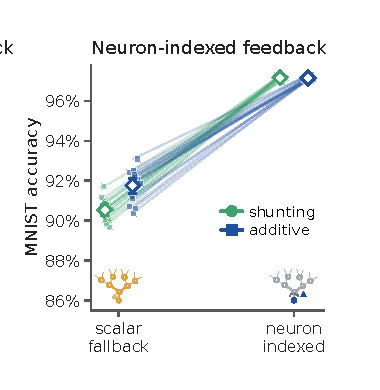
\includegraphics[width=\linewidth,height=4.75cm,keepaspectratio]{pdf_assets/identity_panel_b.pdf}\par
      {\scriptsize\color{Mute}15-seed regular-tree replication shown; the
       range and 120/120 pairs are the prospective 640-run cohort\par}
    \end{column}
  \end{columns}
  \vfill
  \takeaway{Per-neuron bandwidth, not routing --- the classic bottleneck (Werfel--Xie--Seung 2005).}
  \vspace{0.04cm}
\end{frame}

% 21 — ownership
\begin{frame}{Correct ownership adds a small, reproducible margin}
  \begin{columns}[T,onlytextwidth]
    \begin{column}{0.44\textwidth}
      \centering
      \vspace{0.06cm}
      \DerangedPair[0.56]\par
      \eqstrip{\widehat\delta^{\,\mathrm{deranged}}_u=\delta_{0,\pi(u)}}
      \raggedright
      \headline[Add]{$+0.15$ to $+0.70$ pp}{correct neuron-to-tree map,
        favored in 58/60 valid pairs --- same values, same bandwidth}
    \end{column}
    \begin{column}{0.52\textwidth}
      \centering
      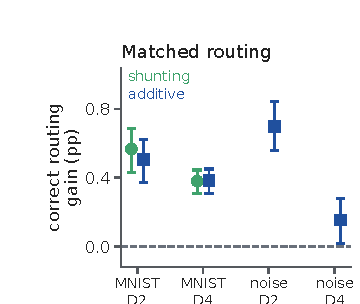
\includegraphics[width=\linewidth,height=4.30cm,keepaspectratio]{pdf_assets/ownership_margin.pdf}\par
      {\scriptsize\color{Mute}identity buys points; ownership, fractions\par}
    \end{column}
  \end{columns}
  \vfill
  \takeaway{Identity is mostly bandwidth; owning the right tree adds a small, real margin.}
  \vspace{0.04cm}
\end{frame}

% 22 — subtree address factorial
\begin{frame}{Subtree addresses win only at the predicted budget}
  \begin{columns}[T,onlytextwidth]
    \begin{column}{0.42\textwidth}
      \centering
      \vspace{0.10cm}
      \CreditTree[mode=address,K=4,scale=0.86,stagelabel={$K$ nested route fields}]\par
      \raggedright
      \headline[Dend]{$+1.3$ pp at $K{=}4$}{only at the predicted budget
        (15/20 seeds, $P{=}0.0048$); 2,700 matched fits}
    \end{column}
    \begin{column}{0.54\textwidth}
      \centering
      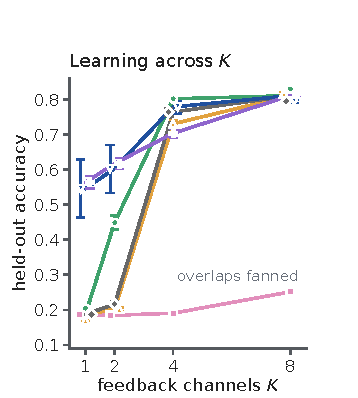
\includegraphics[width=\linewidth,height=4.80cm,keepaspectratio]{pdf_assets/subtree_k_sweep.pdf}\par
      {\scriptsize\color{Mute}$K{=}1,2$ lose, $K{=}8$ ties --- the crossover
       lands where the theory put it\par}
    \end{column}
  \end{columns}
  \vfill
  \takeaway{An interior optimum in feedback bandwidth --- observed where predicted.}
  \vspace{0.04cm}
\end{frame}

% 23 — alignment and depth phase
\begin{frame}{Depth pays when route scales match the task hierarchy}
  \begin{columns}[T,onlytextwidth]
    \begin{column}{0.42\textwidth}
      \centering
      \vspace{0.10cm}
      \CreditTree[mode=address,K=4,scale=0.80,stagelabel={signal at levels $\leq H$, noise below}]\par
      \raggedright
      \headline[Dend]{$+27.7$ pp}{final step of the alignment dose
        (D3$-$D1); optimal routed depth $=H$ for every $H$}
    \end{column}
    \begin{column}{0.54\textwidth}
      \centering
      % single anchor: panel N alone (depth benefit vs sensor alignment);
      % the accuracy curves and dose contrasts (journal panels M, O) live in
      % the speaker notes.
      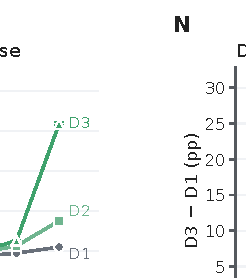
\includegraphics[width=\linewidth,height=4.85cm,keepaspectratio]{pdf_assets/depth_benefit_n.pdf}\par
      {\scriptsize\color{Mute}controlled validation under an imposed
       hierarchy --- not a discovery about arbitrary tasks\par}
    \end{column}
  \end{columns}
  \vfill
  \takeaway{Alignment is a steep boundary the data cross --- not a linear dose.}
  \vspace{0.04cm}
\end{frame}

% 24 — physical depth
\begin{frame}{Aligned divisive depth helps; depth per se costs}
  \begin{columns}[T,onlytextwidth]
    \begin{column}{0.44\textwidth}
      \centering
      \vspace{0.04cm}
      \begin{tikzpicture}[line cap=round]
        \foreach \i/\lab/\stg in {0/{D1}/1,1.35/{D2}/2,2.70/{D3}/3}{
          \begin{scope}[shift={(\i,0)}]
            \filldraw[fill=Soma,draw=Ink!30,line width=0.5pt] (0,0) circle (0.115);
            \foreach \s in {1,...,\stg}{
              \node[rounded corners=1.4pt,draw=Dend,fill=ShuntPale,
                    line width=0.6pt,minimum width=0.44cm,minimum height=0.17cm,
                    inner sep=0pt] at (0,0.30+0.34*\s-0.34) {};
              \draw[Dend,line width=0.8pt] (0,0.115) -- (0,0.215);}
            \node[font=\tiny,text=Mute,anchor=north] at (0,-0.22) {\lab};
          \end{scope}}
      \end{tikzpicture}\par
      \eqstrip{V_n=\frac{E_n+C_n}{1+E_n+I_n+G_n+\epsilon}}
      \raggedright
      \headline[Shunt]{$+31$ pp}{aligned D3$-$D1, constructed; controls
        $\approx0$; depth alone costs (40/40)}
    \end{column}
    \begin{column}{0.52\textwidth}
      \centering
      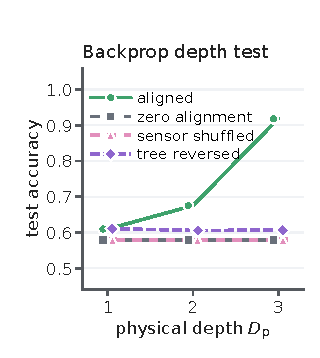
\includegraphics[width=\linewidth,height=4.85cm,keepaspectratio]{pdf_assets/physical_depth_headline.pdf}\par
      {\scriptsize\color{Mute}same branch units and parameters at every
       depth; aligned composition rises, every control stays flat\par}
    \end{column}
  \end{columns}
  \vfill
  \takeaway{A constructed existence proof --- conditional on alignment, never free.}
  \vspace{0.04cm}
\end{frame}

% 25 — real arbors as dictionaries
\begin{frame}{Real arbors are sparse, coarse route dictionaries}
  \begin{columns}[T,onlytextwidth]
    \begin{column}{0.40\textwidth}
      \centering
      \vspace{0.10cm}
      \CreditTree[mode=address,K=8,scale=0.92,stagelabel={ancestry dictionary, 8 channels}]\par
      \raggedright
      \headline[Shunt]{$2.7\times$}{anatomy-specific capture per wiring,
        beyond a density-matched shuffle --- 8 MICrONS cells}
    \end{column}
    \begin{column}{0.56\textwidth}
      \centering
      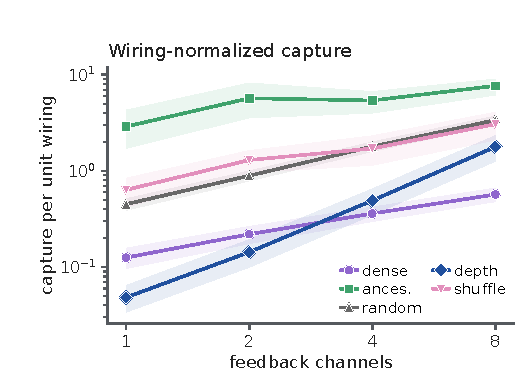
\includegraphics[width=\linewidth,height=4.75cm,keepaspectratio]{pdf_assets/capture_per_wire.pdf}\par
      {\scriptsize\color{Mute}eight sparse ancestry channels reach most of
       dense capture at 7\% of its wiring\par}
    \end{column}
  \end{columns}
  \vfill
  \takeaway{Sparsity does most of the work; anatomy adds a bounded margin on top.}
  \vspace{0.04cm}
\end{frame}

% 26 — shunting mechanism
\begin{frame}{A focal shunt rewrites transport below the branch}
  \begin{columns}[T,onlytextwidth]
    \begin{column}{0.44\textwidth}
      \centering
      \vspace{0.10cm}
      \TreeStrip{\CreditTree[mode=shunt,shunted=false,scale=0.54,stagelabel={baseline}]}%
                {\CreditTree[mode=shunt,shunted=true,scale=0.54,stagelabel={focal inhibition}]}\par
      \raggedright
      \headline[Shunt]{$0.069$}{shunt $-$ additive localization contrast;
        8/8 cells, dose-monotone --- soma and output error matched}
    \end{column}
    \begin{column}{0.52\textwidth}
      \centering
      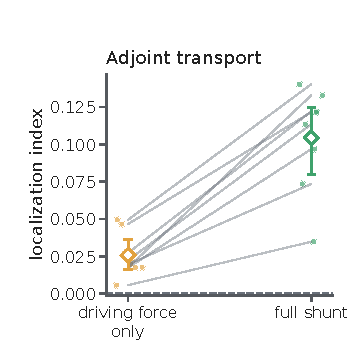
\includegraphics[width=\linewidth,height=4.85cm,keepaspectratio]{pdf_assets/transport_contrast_h.pdf}\par
      {\scriptsize\color{Mute}freezing the adjoint kills the effect;
       restoring it recovers it\par}
    \end{column}
  \end{columns}
  \vfill
  \takeaway{Shunting edits the transported error, not the local driving force.}
  \vspace{0.04cm}
\end{frame}

% 27 — electrotonic boundary
\begin{frame}{The mechanism needs high-conductance states}
  \begin{columns}[T,onlytextwidth]
    \begin{column}{0.42\textwidth}
      \centering
      \vspace{0.10cm}
      \CreditTree[mode=shunt,shunted=true,scale=0.92,stagelabel={a state-dependent operator}]\par
      \raggedright
      \headline[Shunt]{$0.067$}{contrast at in-vivo-like $R_m$ (8/8 cells);
        null at textbook resting calibration}
    \end{column}
    \begin{column}{0.54\textwidth}
      \centering
      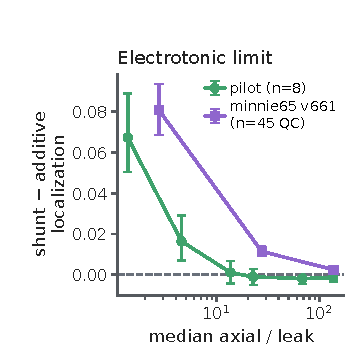
\includegraphics[width=\linewidth,height=4.60cm,keepaspectratio]{pdf_assets/focal_boundary.pdf}\par
      {\scriptsize\color{Mute}active Na/K/Ca/HCN/NMDA ensembles show the same
       contrast --- attenuation only, no sign flips\par}
    \end{column}
  \end{columns}
  \vfill
  \takeaway{State-dependence is the mechanism claim: a testable boundary, not a failure.}
  \vspace{0.04cm}
\end{frame}

% 28 — measured boundary + alignment rescue
\begin{frame}{Anatomy alone is not enough; alignment rescues it}
  \begin{columns}[T,onlytextwidth]
    \begin{column}{0.50\textwidth}
      \vspace{0.10cm}
      \eqstrip{\bm g(a)=\sqrt a\,\bm u_{\parallel}+\sqrt{1-a}\,\bm u_{\perp},
        \ \ \lVert QQ^{\mathsf T}\bm g(a)\rVert^{2}=a}
      {\footnotesize Measured responses give a null --- a boundary, not a
       failure. Rotating alignment rescues the same dictionary.\par}
      \headline[Violet]{$\rho_s=0.99$}{capture predicts 20-step learning;
        $a{=}0$ loses 8/8, $a{=}1$ wins 8/8}
    \end{column}
    \begin{column}{0.46\textwidth}
      \centering
      % single anchor: capture--progress panel; the 20-step learning curves
      % (journal panel M) live in the speaker notes.
      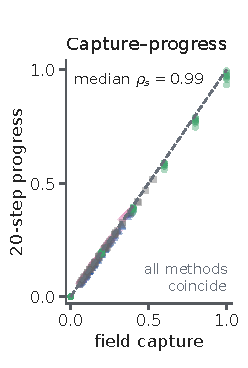
\includegraphics[width=\linewidth,height=4.85cm,keepaspectratio]{pdf_assets/alignment_rescue_n.pdf}\par
      {\scriptsize\color{Mute}same cells, same channels, fixed gradient
       energy and curvature; only alignment rotates\par}
    \end{column}
  \end{columns}
  \vfill
  \takeaway{Alignment, not anatomy alone, determines utility.}
  \vspace{0.04cm}
\end{frame}

% 29 — animal coordinates
\begin{frame}{Animal teaching signals are signed and neuron-specific}
  \begin{columns}[T,onlytextwidth]
    \begin{column}{0.42\textwidth}
      \centering
      \vspace{0.14cm}
      \begin{tikzpicture}[line cap=round]
        \CTminitree{0}{0}
        \CTminitree{2.05}{0}
        \node[font=\scriptsize\bfseries,text=Shunt,anchor=north] at (0.02,-0.28) {P$^{+}$};
        \node[font=\scriptsize\bfseries,text=BP,anchor=north] at (2.07,-0.28) {P$^{-}$};
        \draw[Shunt,-{Stealth[length=4pt]},line width=1.0pt] (0.95,0.45) -- (0.95,1.15);
        \draw[BP,-{Stealth[length=4pt]},line width=1.0pt] (3.00,1.15) -- (3.00,0.45);
        \node[font=\tiny,text=Shunt,anchor=south] at (0.95,1.22) {$+$};
        \node[font=\tiny,text=BP,anchor=north] at (3.00,0.38) {$-$};
      \end{tikzpicture}\par
      \vspace{0.10cm}
      {\scriptsize\color{Mute}opposite causal signs, fixed by the BCI
       mapping, predict opposite dendritic contrasts\par}
      \raggedright
      \headline[Add]{$83.7\%$}{of contrast energy in the signed,
        neuron-specific mode --- 6/6 animals}
    \end{column}
    \begin{column}{0.54\textwidth}
      \centering
      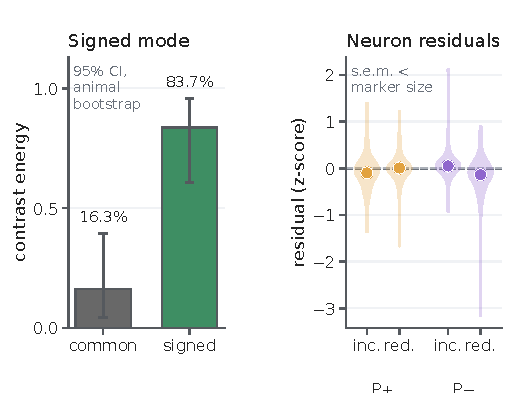
\includegraphics[width=\linewidth,height=4.45cm,keepaspectratio]{pdf_assets/animal_signed.pdf}\par
      {\scriptsize\color{Mute}six-animal reanalysis of published source data
       (Francioni et al., Nature 2026); it does not resolve within-tree
       transport\par}
    \end{column}
  \end{columns}
  \vfill
  \takeaway{The coordinate rung exists in vivo; transport is the open measurement.}
  \vspace{0.04cm}
\end{frame}

% 30 — ACT V divider
\begin{frame}[t]
  \vspace{1.55cm}
  {\color{Shunt}\bfseries\scriptsize ACT V\par}
  \vspace{0.30cm}
  {\fontsize{20}{25}\selectfont\bfseries\color{Ink}What does this teach about\\[0.04cm]learning in the brain?\par}
  \vspace{0.28cm}
  {\small\color{Mute}One phase plane, four inequalities, wiring economics, testable predictions\par}
  \vfill
  \hfill\stackmotif{4}\par
  \vspace{0.12cm}
\end{frame}

% ===========================================================================
% ACT V — What this teaches about brain learning
% ===========================================================================

% 31 — summary phase plane
\begin{frame}{Alignment $\times$ bandwidth decides when structure pays}
  \begin{columns}[T,onlytextwidth]
    \begin{column}{0.58\textwidth}
      \centering
      % talk crop: figure-internal legend and Source-Data footnotes removed
      % at export; the tikz column on the right is the single legend.
      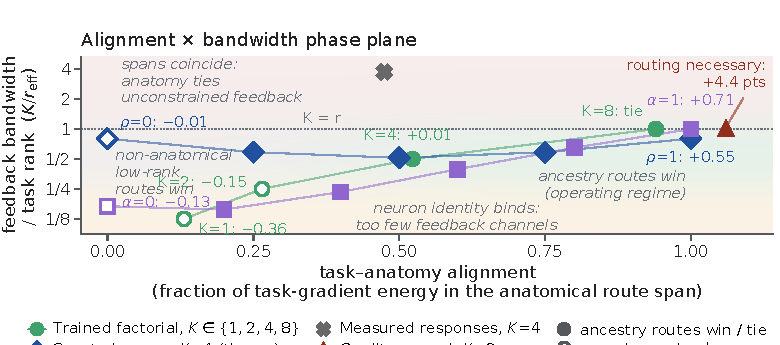
\includegraphics[width=\linewidth,height=5.45cm,keepaspectratio]{pdf_assets/phase_plane.pdf}
    \end{column}
    \begin{column}{0.38\textwidth}
      \footnotesize
      \vspace{0.30cm}
      {\color{Dend}\raisebox{0.1ex}{$\bullet$}}\enspace trained address
      factorial: interior win\par
      \vspace{0.14cm}
      {\color{Add}$\blacklozenge$}\enspace spectral sweep: alignment rotates
      the advantage in\par
      \vspace{0.14cm}
      {\color{Violet}$\blacksquare$}\enspace MICrONS controlled fields\par
      \vspace{0.14cm}
      {\color{Mute}$\boldsymbol\times$}\enspace measured responses: spans
      coincide, predicted null\par
      \vspace{0.14cm}
      {\color{BP}$\blacktriangle$}\enspace credit reversal: routing becomes
      necessary\par
      \vspace{0.16cm}
      {\scriptsize\color{Mute}open marker $=$ anatomical routes lose\par}
    \end{column}
  \end{columns}
  \vfill
  \takeaway{Alignment and bandwidth organize every result on one plane.}
  \vspace{0.04cm}
\end{frame}

% 32 — four comparisons
\begin{frame}{When a local rule wins is settled by four inequalities}
  \vspace{0.10cm}
  \deftag{ceiling}\enspace{\small $M=I,\ \Sigma=0$}\enspace
  {\footnotesize\color{Mute}nothing beats exact BP at matched step norm\par}
  \vspace{0.06cm}{\color{Grid}\rule{\textwidth}{0.35pt}\par}\vspace{0.10cm}
  \deftag{noise}\enspace{\small
    $\tr[(I-P)\Sigma]>\lVert(I-P)\bm g\rVert_2^{2}$}\enspace
  {\footnotesize\color{Mute}beat stochastic BP by rejecting noise\par}
  \vspace{0.06cm}{\color{Grid}\rule{\textwidth}{0.35pt}\par}\vspace{0.10cm}
  \deftag{span}\enspace{\small leading rank-$K$ eigenspace
    $\subset$ ancestry span}\enspace
  {\footnotesize\color{Mute}anatomy is Ky--Fan optimal only under
   alignment\par}
  \vspace{0.06cm}{\color{Grid}\rule{\textwidth}{0.35pt}\par}\vspace{0.10cm}
  \deftag{address}\enspace{\small
    $\cos(g^{\mathrm{shared}},g^{\mathrm{exact}})
      =1/\sqrt{1+\mathrm{CV}_w(\widetilde\alpha)^{2}}<1$}\enspace
  {\footnotesize\color{Mute}addresses win once transport varies\par}
  \vfill
  \takeaway{Structure never beats the exact first-order ceiling; it pays only under alignment.}
  \vspace{0.04cm}
\end{frame}

% 33 — wiring economics
\begin{frame}{Why dendrites: one arbor multiplexes $K$ channels}
  \begin{columns}[T,onlytextwidth]
    \begin{column}{0.44\textwidth}
      \centering
      \vspace{0.10cm}
      \CreditTree[mode=address,K=4,scale=0.82,stagelabel={one neuron, $K$ routed teaching channels}]\par
      \vspace{0.16cm}
      \begin{tikzpicture}[line cap=round]
        \foreach \x/\c in {0/Shunt,1.05/Add,2.10/Amber,3.15/Violet}{
          \filldraw[fill=Soma,draw=Ink!30,line width=0.5pt] (\x,0) circle (0.14);
          \draw[\c,-{Stealth[length=3.5pt]},line width=0.9pt]
            (\x,0.68) -- (\x,0.22);
        }
        \node[font=\tiny,text=Mute,anchor=north] at (1.58,-0.26)
          {or: $K$ point neurons, $K\times$ the feedback wiring};
      \end{tikzpicture}\par
    \end{column}
    \begin{column}{0.52\textwidth}
      \eqstrip{\operatorname{rank}(\Phi_{T,K})\leq K}
      {\footnotesize A point system pays for the same addresses with routed
       coefficients, gated parameter groups, or extra units.\par}
      \headline[Shunt]{$6.9\%$}{of dense-oracle wiring buys 85\% of its
        capture --- $K{=}8$ ancestry channels, reconstructed cells}
    \end{column}
  \end{columns}
  \vfill
  \takeaway{Dendrites relocate address resources; the ledger is wiring.}
  \vspace{0.04cm}
\end{frame}

% 34 — predictions
\begin{frame}{The theory is testable with focal dendritic inhibition}
  \begin{columns}[T,onlytextwidth]
    \begin{column}{0.58\textwidth}
      \vspace{0.10cm}
      \deftag{prediction 1}\par
      {\footnotesize plasticity shifts below the branch\par}
      \vspace{0.18cm}
      \deftag{prediction 2}\par
      {\footnotesize scales with dose and $R_{\mathrm{in}}$; saturates\par}
      \vspace{0.18cm}
      \deftag{prediction 3}\par
      {\footnotesize needs high-conductance states\par}
      \vspace{0.18cm}
      \deftag{prediction 4}\par
      {\footnotesize tracks capture, not morphology\par}
    \end{column}
    \begin{column}{0.38\textwidth}
      \centering
      \CreditTree[mode=shunt,shunted=true,scale=0.98,stagelabel={focal dendritic inhibition}]
    \end{column}
  \end{columns}
  \vfill
  \takeaway{Branch-resolved plasticity separates credit routing from gain control.}
  \vspace{0.04cm}
\end{frame}

% 35 — closing: the four act questions, answered
\begin{frame}{Four questions, four answers}
  \begin{columns}[T,onlytextwidth]
    \begin{column}{0.62\textwidth}
      \vspace{0.10cm}
      {\scriptsize\color{Mute}ACT II\par}
      {\small\bfseries One signed coordinate per neuron.\par}
      \vspace{0.26cm}
      {\scriptsize\color{Mute}ACT III\par}
      {\small\bfseries Eligibility $\times$ transported, routed error.\par}
      \vspace{0.26cm}
      {\scriptsize\color{Mute}ACT IV\par}
      {\small\bfseries Yes --- at the predicted budget, under alignment.\par}
      \vspace{0.26cm}
      {\scriptsize\color{Mute}ACT V\par}
      {\small\bfseries One phase plane organizes every result.\par}
    \end{column}
    \begin{column}{0.34\textwidth}
      \centering
      \vspace{0.30cm}
      \scalebox{1.5}{\stackmotif{4}}\par
      \vspace{0.55cm}
      {\scriptsize\color{Mute}Thanks: Sabatini and Richards labs, Kempner
       Institute compute and support.\par}
    \end{column}
  \end{columns}
  \vfill
  \takeaway{Coordinates name neurons; trees address synapses; conductance tunes gain; alignment decides value.}
  \vspace{0.04cm}
\end{frame}
